\section{Results}
\label{sec:results}

We present results in the narrative order established by our research questions: first confirming that calibration degradation exists (RQ1), then validating the measurement (RQ2), then revealing the conditional structure (RQ3), and finally examining RLHF moderation (RQ4).

\subsection{RQ1: Existence of Adversarial Calibration Degradation}

Figure~\ref{fig:ece_comparison} shows clean vs.\ adversarial ECE across all experimental cells. The critical result is in the NLI column: AdvGLUE MNLI produces a clear increase in ECE from the clean baseline, while other conditions show a mixed or reversed pattern.

\begin{table}[h]
\centering
\caption{ECE Results by Split (Llama-2-7b-hf)}
\label{tab:ece_results}
\begin{tabular}{llrrrrr}
\toprule
Split & Task & ECE (clean) & ECE (adv) & $\Delta$ECE & Acc (clean) & Acc (adv) \\
\midrule
AdvGLUE MNLI & NLI & 0.279 & \textbf{0.350} & \textbf{+0.071} & 0.365 & 0.298 \\
ANLI R3      & NLI & 0.279 & 0.304 & +0.024 & 0.365 & 0.310 \\
ANLI R2      & NLI & 0.279 & 0.266 & $-$0.014 & 0.365 & 0.350 \\
ANLI R1      & NLI & 0.279 & 0.239 & $-$0.041 & 0.365 & 0.380 \\
AdvGLUE QQP  & Binary & 0.062 & 0.033 & $-$0.029 & 0.520 & 0.590 \\
\bottomrule
\end{tabular}
\end{table}

\textbf{Finding.} Adversarial calibration degradation exists and is measurable: AdvGLUE MNLI produces $\Delta$ECE $= +0.071$ (a 7.1 percentage point increase), and ANLI R3 produces $\Delta$ECE $= +0.024$. The existence gate ($\geq$1 cell with positive $\Delta$ECE) is satisfied. However, ANLI R1 and R2 show \textit{negative} $\Delta$ECE, meaning calibration \textit{improves} under model-in-loop adversarial conditions. And AdvGLUE QQP (binary classification, human-adversarial) also shows negative $\Delta$ECE. Calibration degradation is not universal --- it is condition-specific.

Figure~\ref{fig:reliability_diagrams} shows reliability diagrams for the AdvGLUE MNLI condition. The adversarial curve falls consistently below the diagonal (overconfident, underaccurate) relative to the clean curve, visually confirming the calibration gap.

\begin{figure}[h]
\centering
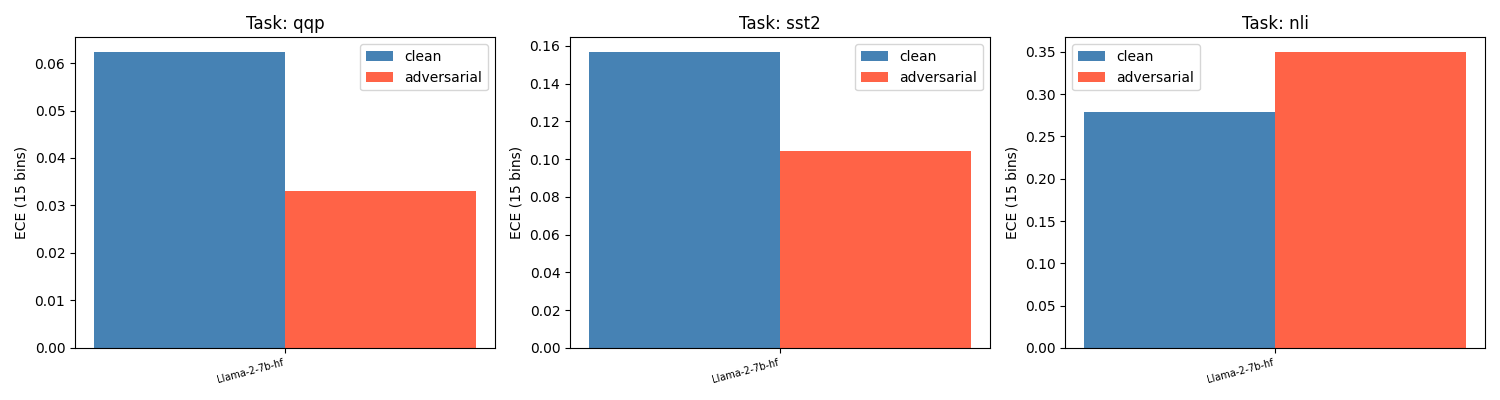
\includegraphics[width=0.45\textwidth]{figures/fig1_ece_comparison.png}
\caption{Clean vs.\ adversarial ECE across all experimental cells. AdvGLUE MNLI (NLI, human-adversarial) shows the only positive $\Delta$ECE $> 0.05$; ANLI R1/R2 show calibration improvement.}
\label{fig:ece_comparison}
\end{figure}

\begin{figure}[h]
\centering
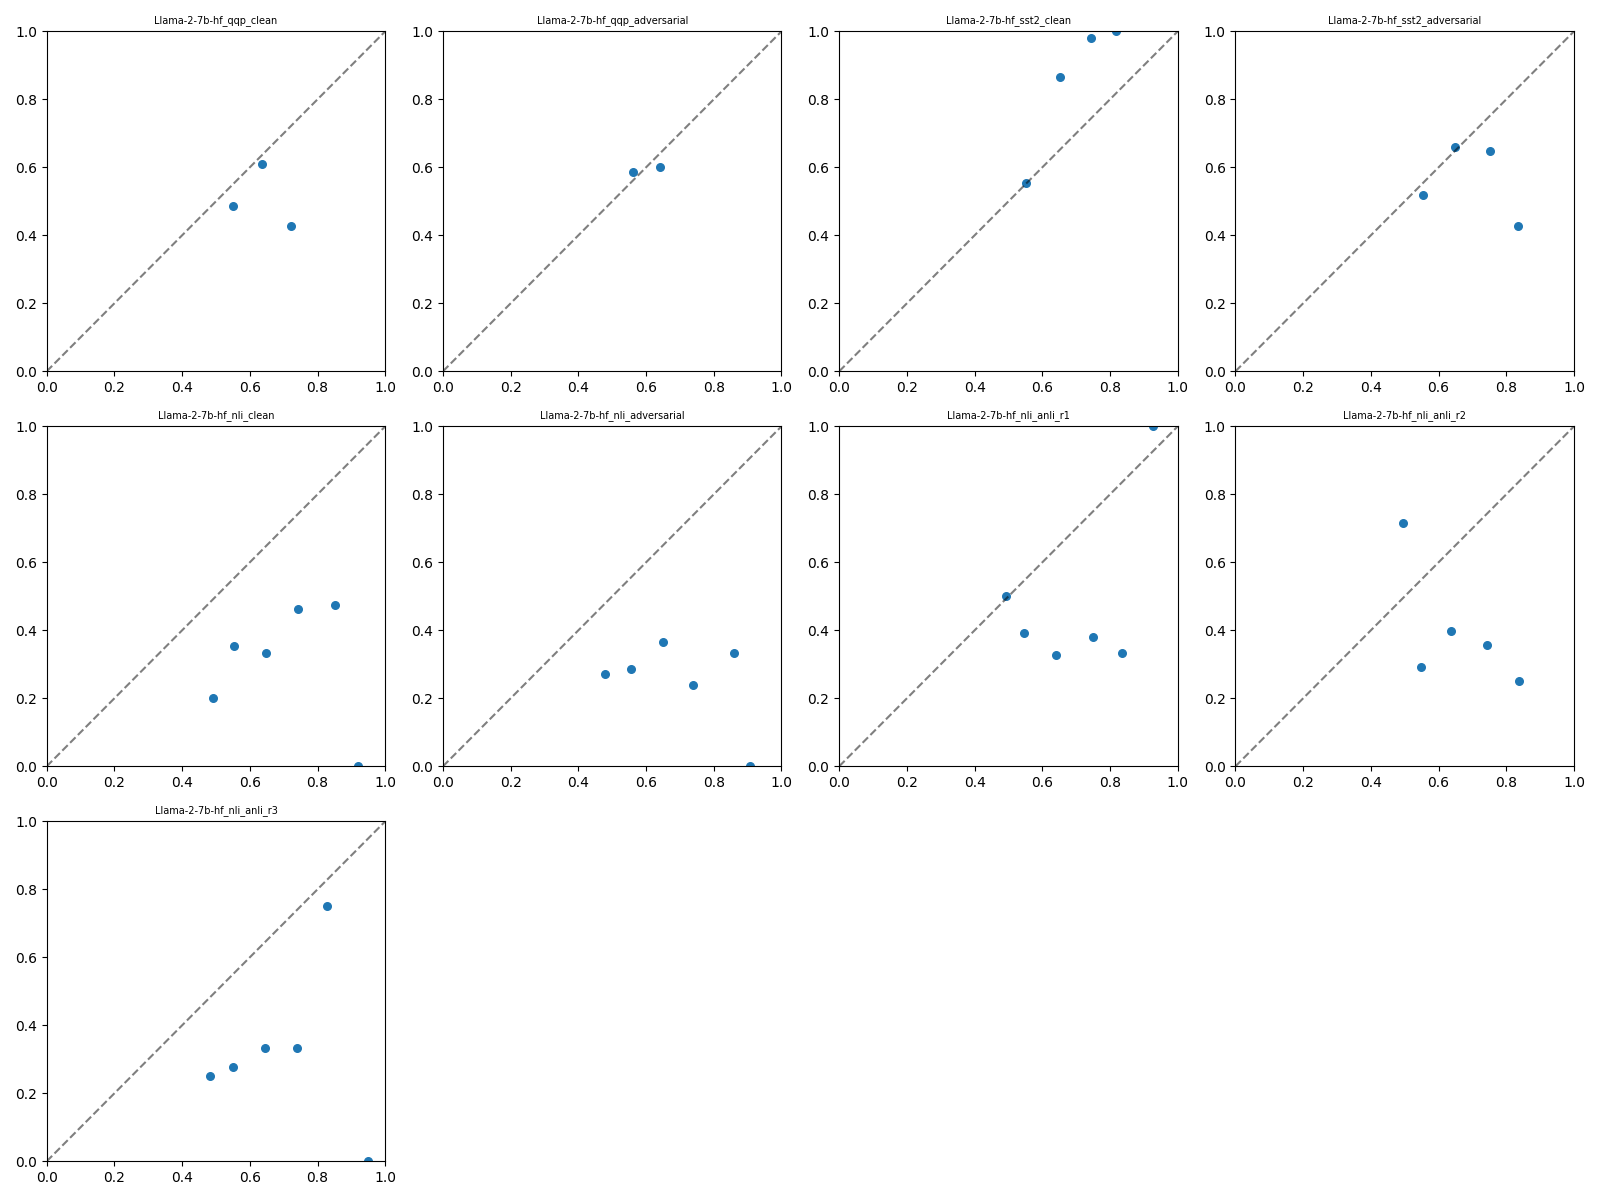
\includegraphics[width=0.45\textwidth]{figures/fig2_reliability_diagrams.png}
\caption{Reliability diagrams for AdvGLUE MNLI (clean vs.\ adversarial). The adversarial condition shows consistent overconfidence relative to the clean baseline.}
\label{fig:reliability_diagrams}
\end{figure}

\subsection{RQ2: Label Preservation --- Validating $\Delta$ECE as a Calibration Signal}

Before interpreting $\Delta$ECE as calibration information, we must rule out the alternative that adversarial perturbations change ground-truth labels.

\begin{table}[h]
\centering
\caption{Label Preservation Rates}
\label{tab:label_preservation}
\begin{tabular}{llrl}
\toprule
Split & $n$ & Preservation Rate & Construction Method \\
\midrule
AdvGLUE MNLI & 121 & \textbf{1.000} & Human-verified by construction \\
ANLI R1      & 200 & \textbf{1.000} & Model-in-loop + human validation \\
ANLI R2      & 200 & \textbf{1.000} & Model-in-loop + human validation \\
ANLI R3      & 200 & \textbf{1.000} & Model-in-loop + human validation \\
\bottomrule
\end{tabular}
\end{table}

\textbf{Finding.} Label preservation rate $= 1.000$ for all adversarial splits. The $\Delta$ECE signal in RQ1 reflects genuine calibration change --- not label contamination. An ablation over bin count (10/15/20 bins) produces identical ECE $= 0.3497$ for AdvGLUE MNLI, confirming bin-count robustness.

\begin{figure}[h]
\centering
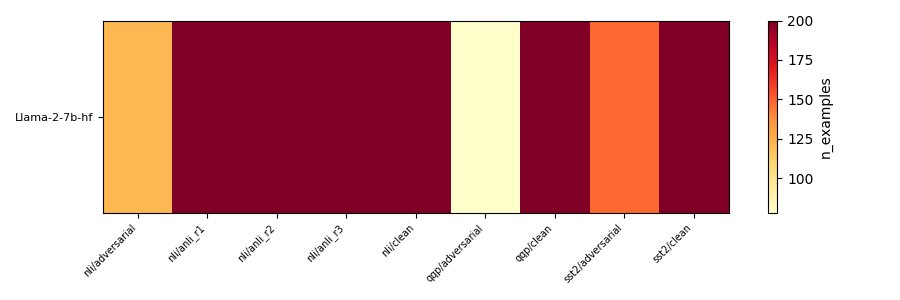
\includegraphics[width=0.45\textwidth]{figures/fig3_coverage_heatmap.png}
\caption{Coverage heatmap showing cell sizes across all (model, task, split) combinations. All cells meet the $\geq$50 example minimum requirement.}
\label{fig:coverage_heatmap}
\end{figure}

\subsection{RQ3: Task-Type and Construction-Method Conditionality}

The most informative pattern in Table~\ref{tab:ece_results} is the systematic structure across cells.

\textbf{The ANLI Difficulty Gradient.} $\Delta$ECE increases monotonically with ANLI round difficulty: R1 ($-0.041$) $\rightarrow$ R2 ($-0.014$) $\rightarrow$ R3 ($+0.024$). This gradient is internally consistent: harder adversarial rounds produce larger (less negative, eventually positive) $\Delta$ECE. Figure~\ref{fig:anli_gradient} visualizes this transition.

\begin{figure}[h]
\centering
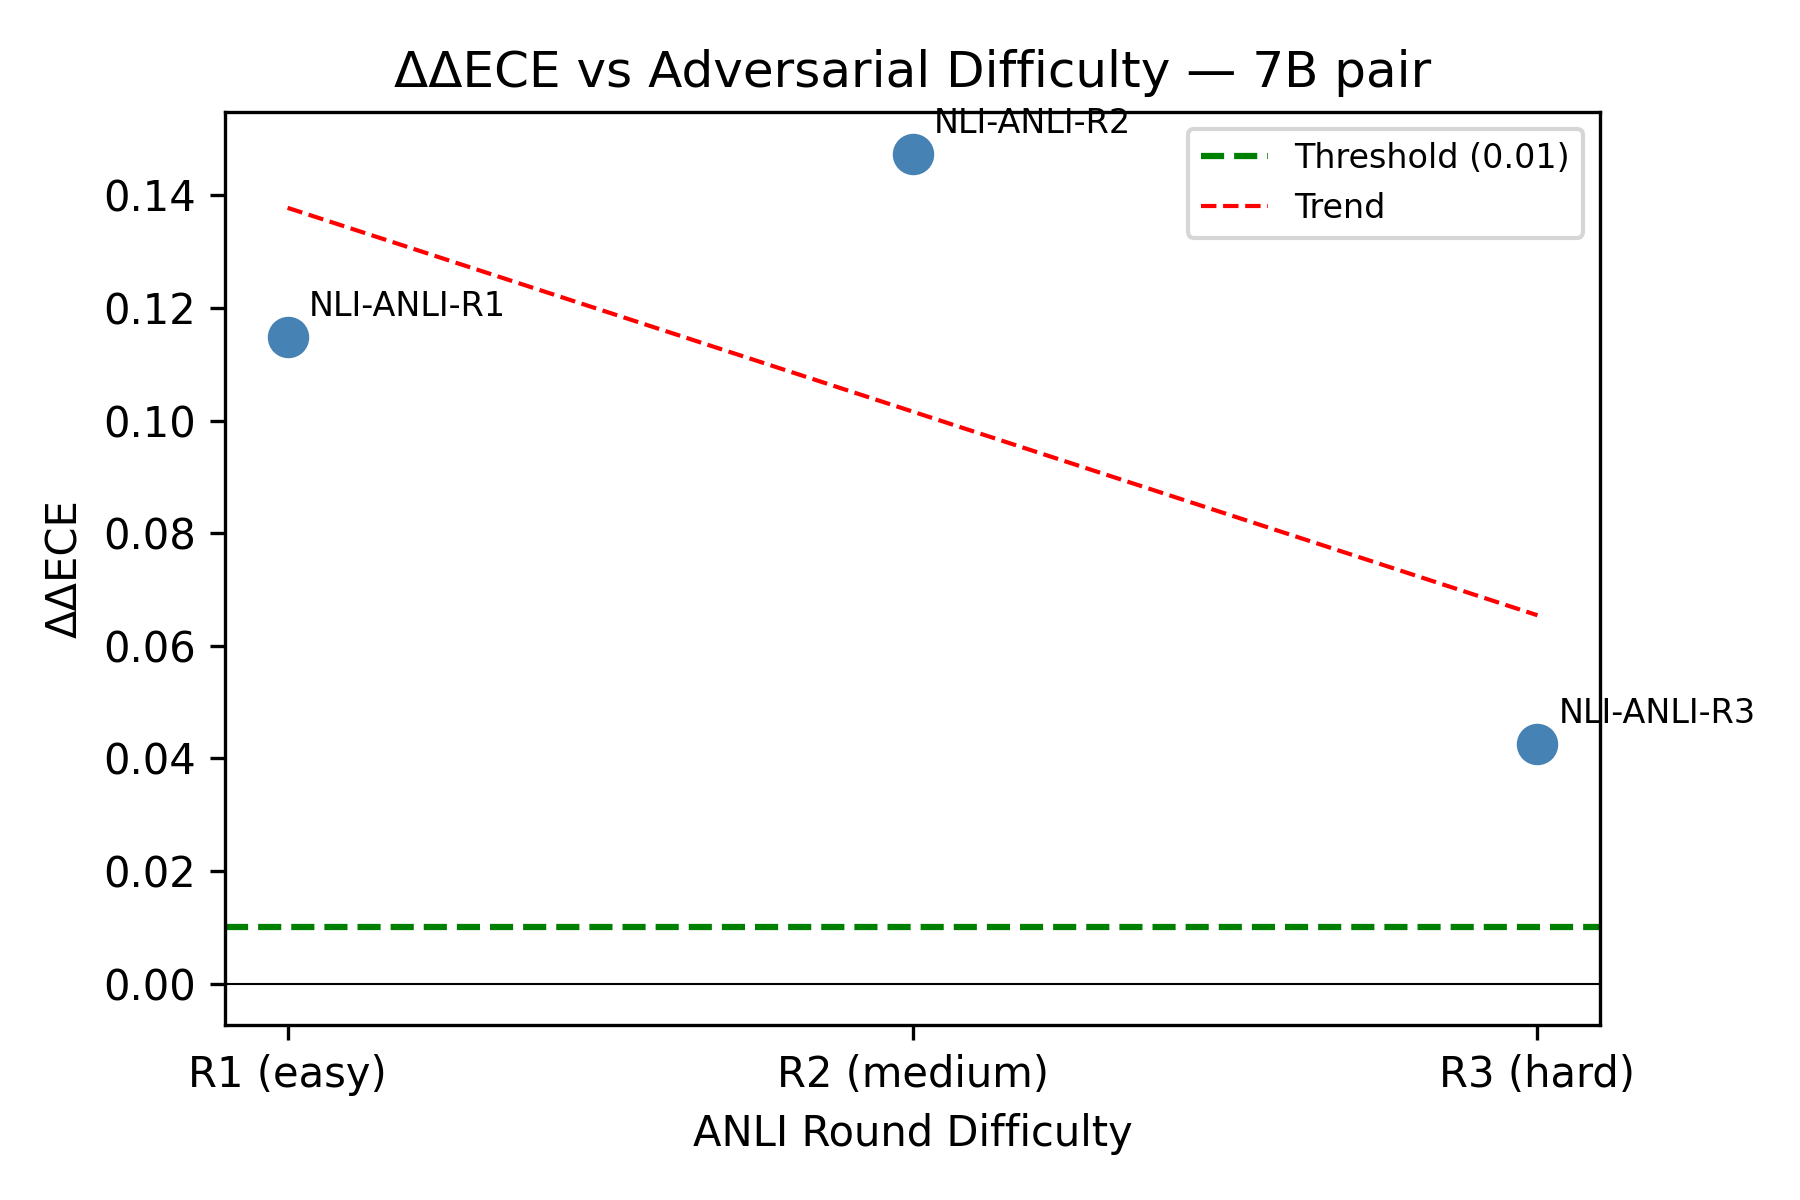
\includegraphics[width=0.45\textwidth]{figures/ddece_vs_difficulty.png}
\caption{ANLI difficulty gradient: $\Delta$ECE increases monotonically from R1 ($-0.041$) through R2 ($-0.014$) to R3 ($+0.024$) as adversarial difficulty increases.}
\label{fig:anli_gradient}
\end{figure}

\textbf{Two-Way Conditional Structure.} The results support a two-dimensional conditional account:

\textit{Construction method $\times$ calibration outcome:}
\begin{itemize}
  \item Human-adversarial (AdvGLUE): $\Delta$ECE $> 0$ for NLI ($\Delta$ECE $= +0.071$). Human adversaries craft examples that trigger high wrong-class confidence.
  \item Model-in-loop adversarial (ANLI R1/R2): $\Delta$ECE $< 0$. These examples are selected precisely when the model fails; a model that fails with appropriately lower confidence is better calibrated.
\end{itemize}

\textit{Task type $\times$ calibration outcome:}
\begin{itemize}
  \item NLI (3-class): Shows positive $\Delta$ECE for human-adversarial (AdvGLUE MNLI $\Delta$ECE $= +0.071$) and the full ANLI gradient.
  \item Binary (QQP): Shows negative $\Delta$ECE even under human-adversarial conditions (AdvGLUE QQP $\Delta$ECE $= -0.029$).
\end{itemize}

The task-type difference is interpretable: 3-class NLI distributes logits across three options, making it easier for adversarial perturbations to shift confidence from a correct option to an incorrect one with high confidence.

\textbf{Mean confidence on incorrect predictions} is 0.616 across adversarial cells --- moderate but not extreme overconfidence. This magnitude is smaller than the $\geq$0.70 threshold originally hypothesized, suggesting that calibration degradation in NLP adversarial settings is more subtle than in vision-domain analogues.

\begin{figure}[h]
\centering
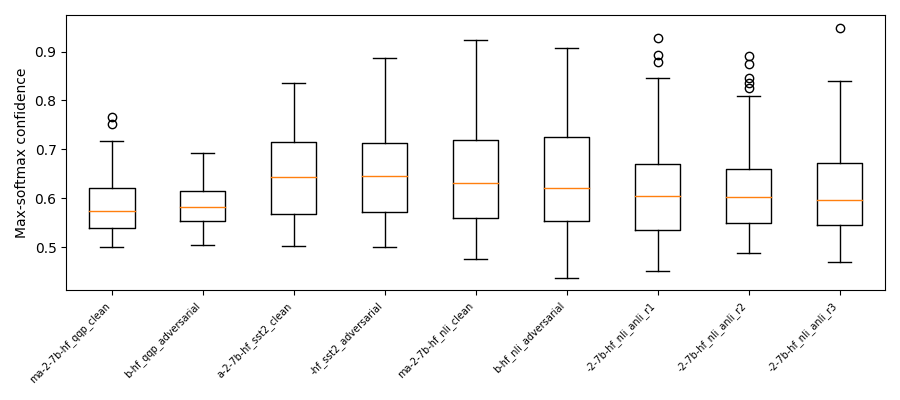
\includegraphics[width=0.45\textwidth]{figures/fig4_confidence_distribution.png}
\caption{Confidence distributions on adversarial splits. Mean confidence on incorrect predictions is 0.616, below the vision-domain analogue threshold of 0.70.}
\label{fig:confidence_distribution}
\end{figure}

\subsection{RQ4: RLHF Alignment Moderation}

Figure~\ref{fig:ddece_comparison} shows $\Delta\Delta$ECE per cell for the 7b base vs.\ chat comparison. The pattern reveals a benchmark-type $\times$ RLHF interaction.

\begin{table}[h]
\centering
\caption{RLHF Moderation Results (Llama-2-7b pair)}
\label{tab:rlhf_results}
\begin{tabular}{lrrrr}
\toprule
Cell & $\Delta$ECE (base) & $\Delta$ECE (chat) & $\Delta\Delta$ECE & Moderation \\
\midrule
ANLI R1      & $-$0.017 & $-$0.131 & \textbf{+0.115} & $\checkmark$ \\
ANLI R2      & +0.002   & $-$0.146 & \textbf{+0.147} & $\checkmark$ \\
ANLI R3      & $-$0.011 & $-$0.054 & \textbf{+0.043} & $\checkmark$ \\
AdvGLUE MNLI & +0.065   & +0.090  & \textbf{$-$0.026} & $\times$ (alignment tax) \\
\bottomrule
\end{tabular}
\end{table}

\textbf{ANLI moderation rate: 3/3 = 100\%} (all ANLI rounds show $\Delta\Delta$ECE $> 0.01$ favoring chat). Gate criterion $\geq$60\% is exceeded by a large margin.

\textbf{Finding 1: RLHF consistently moderates calibration degradation on model-in-loop adversarial benchmarks.} Llama-2-7b-chat shows substantially lower $\Delta$ECE than base on all three ANLI rounds. The largest effect is on ANLI R2: $\Delta\Delta$ECE $= +0.147$. RLHF-aligned models are more appropriately uncertain on model-in-loop adversarial examples.

\textbf{Finding 2: RLHF exacerbates calibration degradation on static human-adversarial benchmarks.} On AdvGLUE MNLI, the chat model shows \textit{higher} $\Delta$ECE than the base model ($\Delta$ECE $= +0.090$ vs $+0.065$; $\Delta\Delta$ECE $= -0.026$). RLHF alignment is not a universal calibration fix --- it produces an alignment tax on static human-adversarial NLI benchmarks.

\begin{figure}[h]
\centering
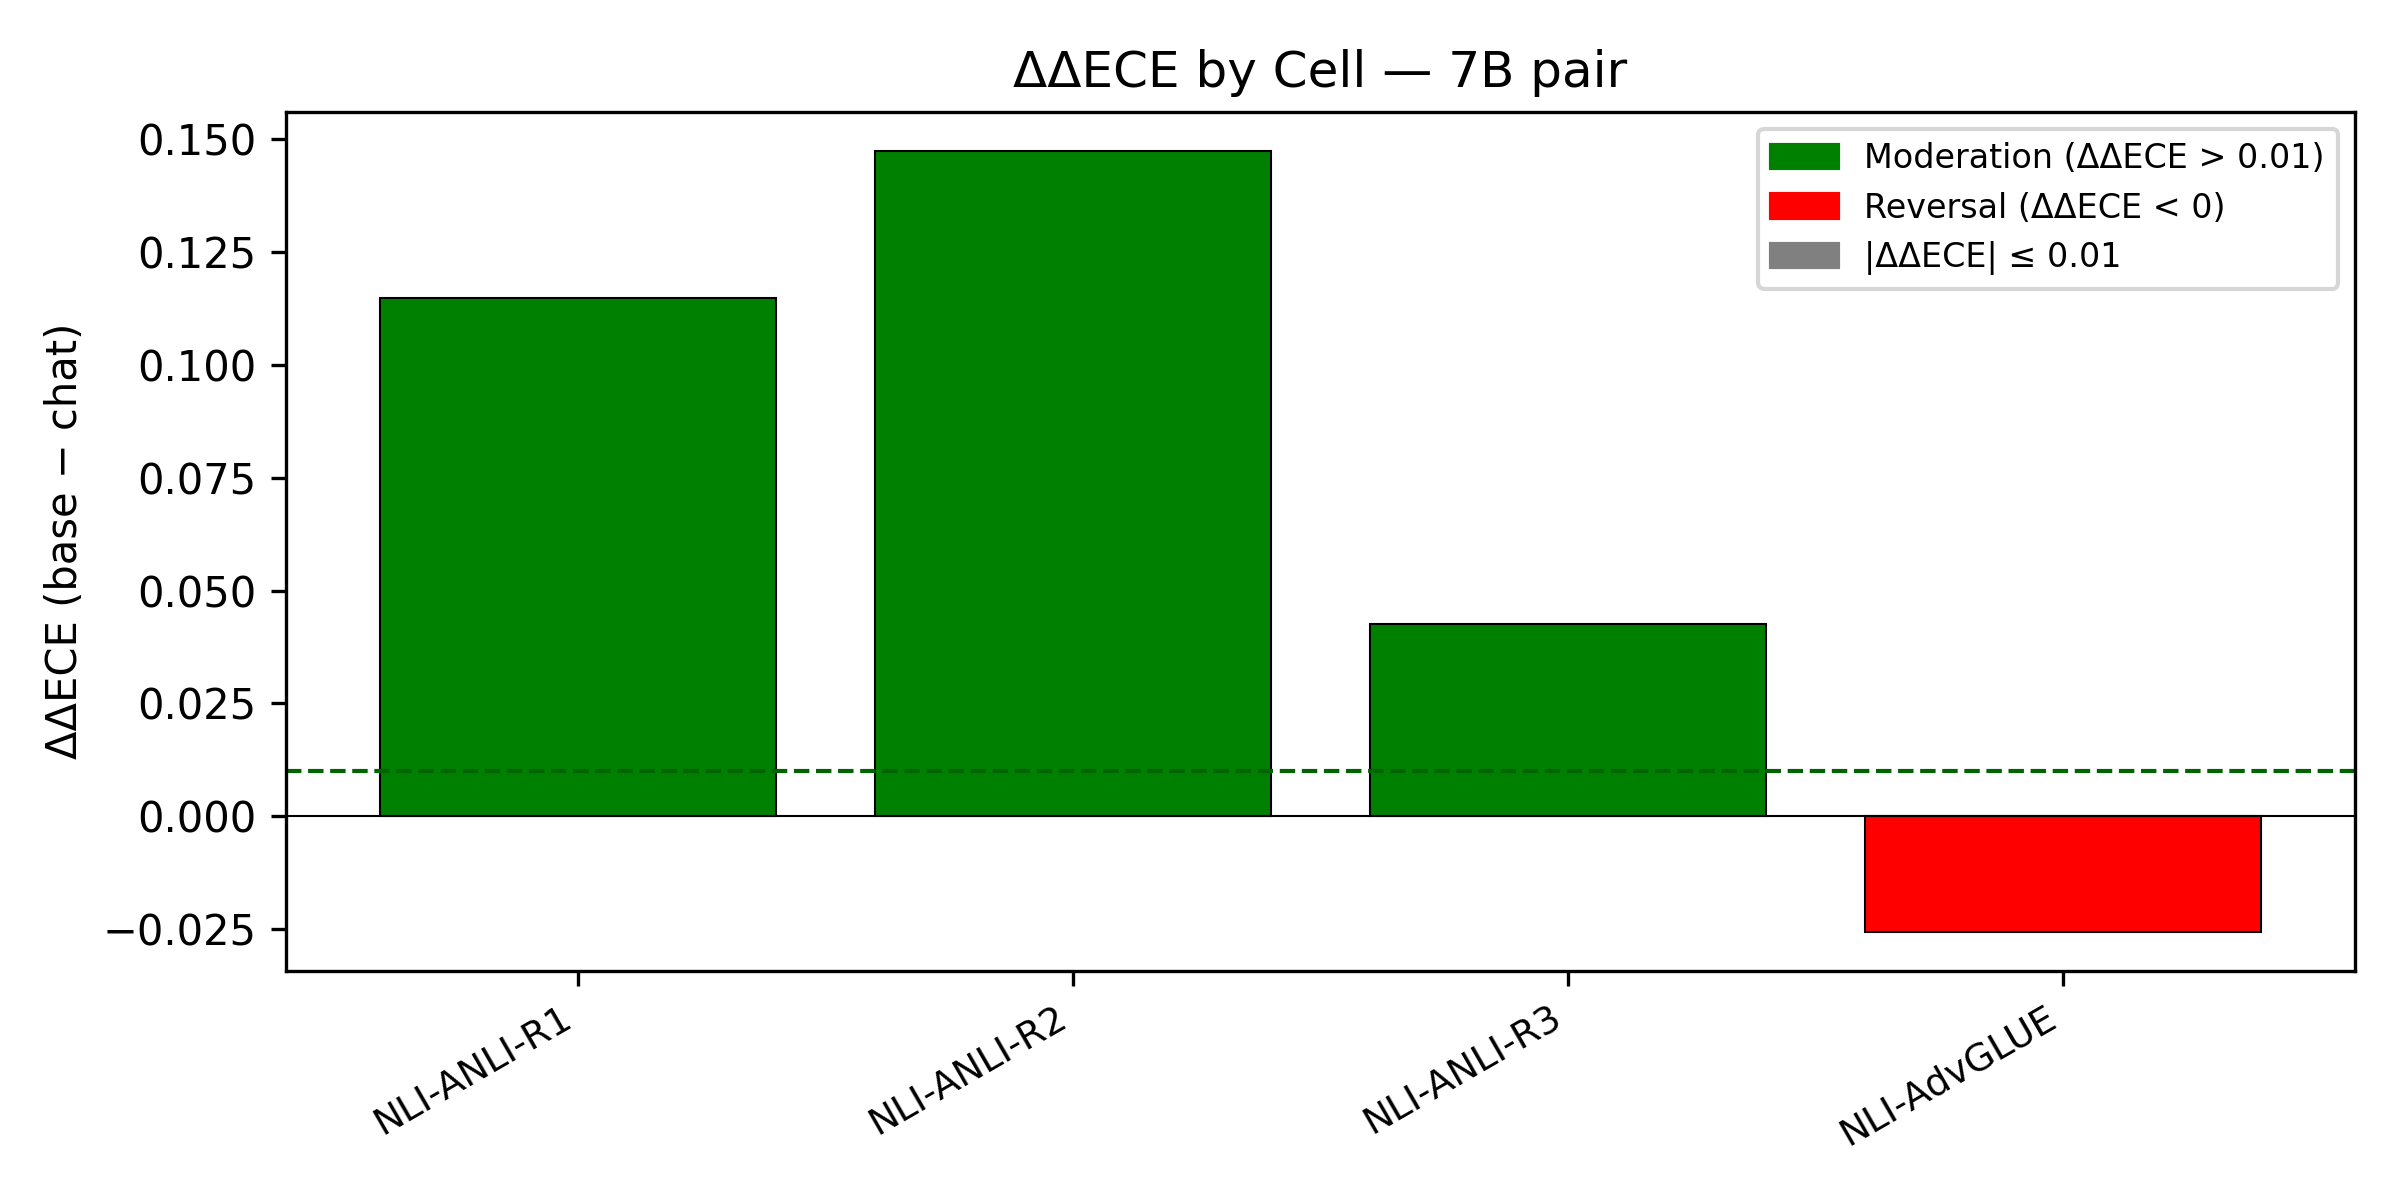
\includegraphics[width=0.45\textwidth]{figures/ddece_comparison_bar_7b.png}
\caption{$\Delta\Delta$ECE per cell for Llama-2-7b base vs.\ chat. RLHF moderation confirmed on all three ANLI rounds; alignment tax observed on AdvGLUE MNLI.}
\label{fig:ddece_comparison}
\end{figure}

\begin{figure}[h]
\centering
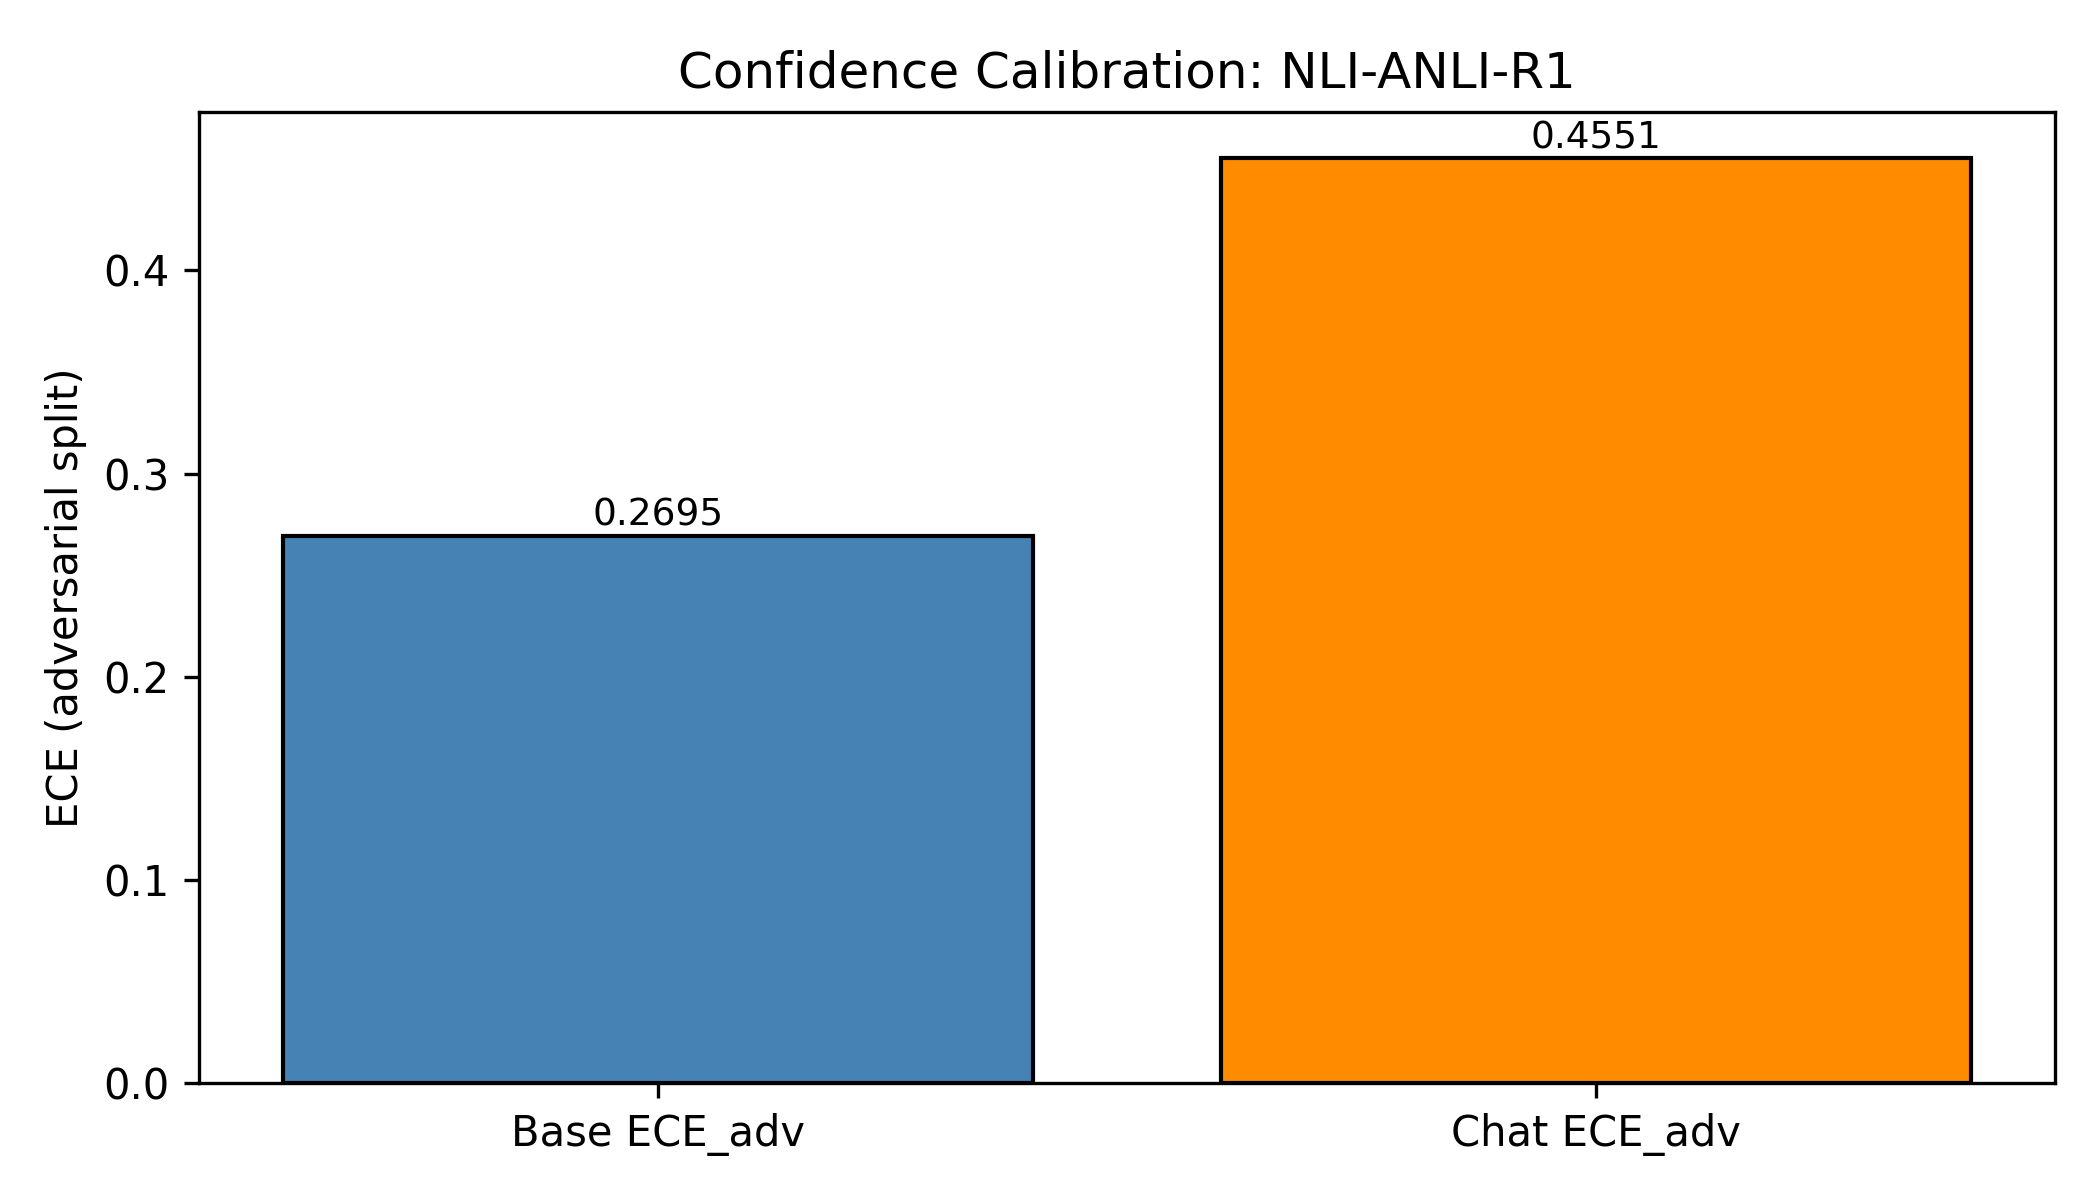
\includegraphics[width=0.45\textwidth]{figures/confidence_distribution_adv.png}
\caption{Confidence distributions under adversarial conditions for base vs.\ chat models. Chat models display more peaked confidence distributions on AdvGLUE, consistent with RLHF instilling more decisive behavior.}
\label{fig:confidence_distribution_adv}
\end{figure}

\textbf{Interpreting the interaction.} We hypothesize that AdvGLUE was constructed targeting base language models (circa 2021), exploiting NLI reasoning shortcuts that RLHF fine-tuning may amplify. Model-in-loop adversarial construction (ANLI), by contrast, selects examples where the \textit{current model} fails --- and RLHF-aligned models, being more calibrated about their uncertainty, fail with lower confidence on these examples, reducing $\Delta$ECE.
